
\begin{figure}[t]  
    \centering
    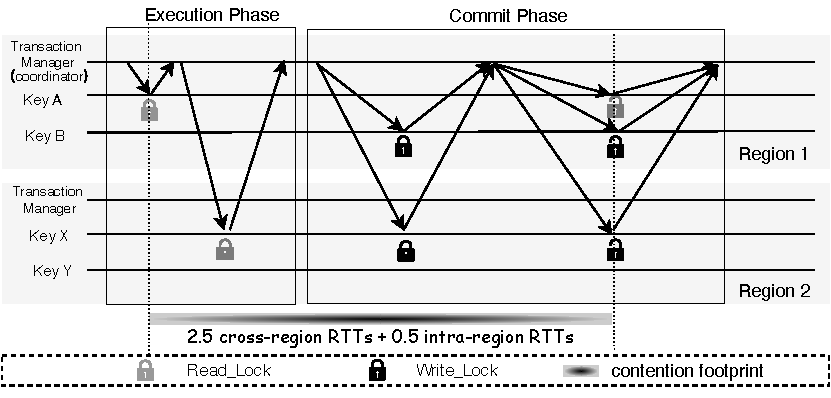
\includegraphics[width=1\columnwidth]{figures/spanner.pdf}
	\vspace{-5pt}
    \caption{This diagram shows how Spanner orders a CRT using 2PL and commits it using 2PC in a multi-region deployment. Replicas are removed for readability.} \label{fig:spanner}
	% \vspace{-5pt}
\end{figure}

\section{\spanner and \spannerxx}\label{sec:spanner}
In this section, we present the design, implementation, and evaluation of Spanner and Spanner-RLS. We regard Spanner-RLS as a specific instance of using our new consistency model (RLS) to advance the performance of existing strictly serializable databases. 

\subsection{Protocols and Implementations}

\noindent\textbf{\spanner Background.} Google's \spanner provides strict serializability (a.k.a. external consistency) for read-write transactions by coordinating them using two-phase locking (2PL) and then committing the transactions using two-phase commit (2PC). 

\fig{fig:spanner} presents an example, where a transaction $T$ reads the keys $A$ and $X$, and then updates the keys $B$ and $X$. The keys $A$ and $B$ are located at different data nodes in $region$ $1$, and the key $X$ is located at a data node in $region$ $2$. To commence, $T$ is forwarded to the transaction manager that $T$ firstly accesses, acting as the coordinator and assigning a globally unique \texttt{TID} to $T$. In this example, the transaction manager of $region$ $1$ serves as the coordinator since $T$ reads the key $A$ in the first access. Subsequently, the coordinator sequentially executes all the transaction operations. During execution, it acquires read locks for each read operation and buffers write operations in temporary memory. After buffering all writes, the coordinator obtains exclusive locks for all write keys (i.e., the keys $B$ and $X$) and installs the writes if all the required locks are acquired. Following this, all the locks (both read and exclusive locks) are released immediately. As such, $T$ is successfully executed and committed.

We are now prepared to introduce the performance issues in Spanner. Spanner coordinates intra-region transactions (IRTs) and cross-region transactions (CRTs) similarly, where a read lock held by a CRT will block all writes from both CRTs and IRTs, and an exclusive lock held by a CRT will prevent all reads and writes, correspondingly. Consequently, a CRT's contention footprint (i.e., the lock duration) is extremely large. More than two cross-region network round trips will block all conflict transactions. In our example, it takes $2.5$ cross-region network round trips and $0.5$ intra-region round trips. Even worse, such blockings can rapidly accumulate through transitive relations. For instance, considering another CRT $T^{\prime}$ that accesses the key $B$ and $Y$, $T^{\prime}$ can successfully acquire the exclusive lock on the key $Y$ while having to wait for the lock on the key $B$. Consequently, all other IRTs and CRTs that access the key $Y$ have to compete with $T^{\prime}$ for ownership of the lock on the key $Y$, enlarging the affected key space.



\begin{figure}[t]  
    \centering
    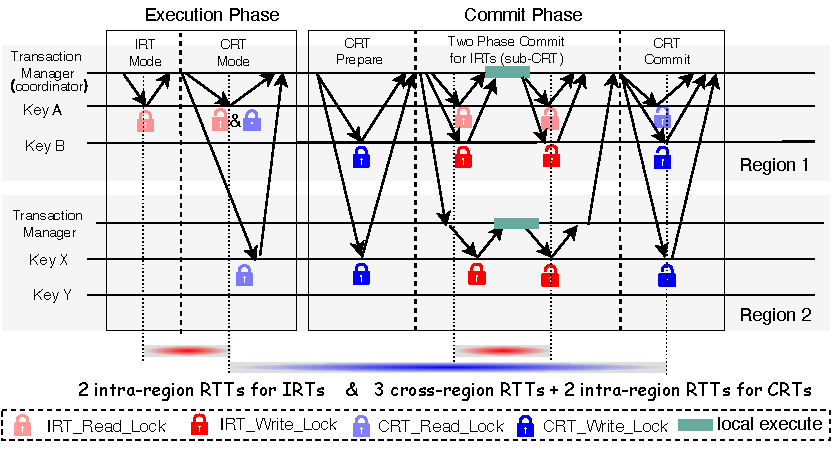
\includegraphics[width=1\columnwidth]{figures/RLS-spanner.pdf}
    \caption{This diagram shows how Spanner-RLS orders a CRT using a variant of 2PL and commits it using 2PC.} \label{fig:spannerrls}
\end{figure}

\SetKwProg{Fn}{function}{:}{}

\SetKwFunction{Coordsp}{Coord-\spxx}
\SetKwFunction{FgetPreLock}{getCrossLock}
\SetKwFunction{FsetPreLock}{setCrossLock}
\SetKwFunction{FgetLock}{getInLock}
\SetKwFunction{FsetLock}{setInLock}
\SetKwFunction{FsendPrepareOK}{sendPrepareOK}
\SetKwFunction{FsendRetry}{sendRetry}
\SetKwFunction{FsendCommitted}{sendCommitted}

\SetKwData{DKey}{key}
\SetKwData{DTxn}{txn}
\SetKwData{PreLock}{crossLock}
\SetKwData{Lock}{inLock}

\SetKwData{UNLOCKED}{unLock}
\SetKwData{RLock}{readLock}
\SetKwData{WLock}{writeLock}
\SetKwData{RWLock}{readWriteLock}
\SetKwData{PreLockHolder}{crossLockHolder}
\SetKwData{LockHolder}{inLockHolder}
\SetKwProg{Event}{Event}{}{end}
\SetKwData{TouchedR}{touchedRegions}

\SetKwData{DRegion}{r}


\begin{algorithm}[t]
	\setstretch{1}
	\small 
  	\Fn{Execution phase}{
      \texttt{read\_set} \&  
      \texttt{write\_set} $\gets \emptyset$ \\
      txnType $\gets$ IRT  \Comment{Start a new transaction as IRT.}\\
       \TouchedR $\gets \emptyset$  \Comment{Regions involved in the transaction.} \\
  \LeftComment{Execute the transaction commands, which triggers the events:}\\
  \Event{$read (\texttt{key}$)}{
    
    $\texttt{value} = find\_record(\texttt{key})$ \\
    $\texttt{read\_set}.append(\texttt{key})$ \\
    \tikzmk{A}
    \TouchedR $\gets$ \TouchedR $\cup$ \texttt{key.region} \\
    \If{$	\lvert \TouchedR 	\rvert \geq 2$}{
      txnType $\gets$ CRT \\
       $Release\_IRT\_Read\_Lock(k)$ $for$ $all$ $k$ $\in$  \texttt{read\_set} \\
       $CRT\_Read\_Lock(k)$ $for$ $all$ $k$ $\in$  \texttt{read\_set} \\
    }
    \uIf{txnType == IRT}{
      $IRT\_Read\_Lock(key)$ \\
    }
    \Else(){
      $CRT\_Read\_Lock(key)$
    }
  }

  \tikzmk{B} \boxit{blue}
  \Event{write (\texttt{key}, \texttt{value}) \Comment{Writes are only buffered }}{
       $\texttt{write\_set}.append(\text{\textless}\texttt{key}, \texttt{value}\text{\textgreater})$ \\
       $Execute \ Line \ 9 \sim 13$ \\
  }

  }
  \renewcommand{\boxit}[1]{\tikz[remember picture,overlay]{\node[xshift=-1.5pt,yshift=0.5pt,fill=#1,opacity=.25,fit={(A)($(B)+(.9\linewidth,.8\baselineskip)$)}] {};}\ignorespaces} 

  \Fn{Commit phase}{
      \uIf{txnType == IRT} {
        $IRT\_Write\_Lock(k)$ $for$ $all$ $k$ $\in$ \texttt{write\_set}  \\
        wait for all \texttt{ACK}s from $storage$ \Comment{Abort if fail} \\ 
        $Commit(txn)$ \\
        $Release\_IRT\_Read\_Lock(k)$ $for$ $all$ $k$ $\in$  \texttt{read\_set} \\
        $Release\_IRT\_Write\_Lock(k)$ $for$ $all$ $k$ $\in$  \texttt{write\_set} \\
      }

      \tikzmk{A} 
      \Else(){
        $CRT\_Write\_Lock(k)$ $for$ $all$ $k$ $\in$ \texttt{write\_set}  \\
        wait for all \texttt{ACK}s from $storage$ \Comment{Abort if fail} \\ 
        Send Commit to $txn$ $managers$ $in$ $r$, $r$ $\in$  \TouchedR  \\
        \LeftComment{Each transaction manager commits the transaction as IRT} \\
        wait for all \texttt{ACK}s from the $txn$ $managers$ \Comment{Abort if fail} \\ 
        $Commit(txn)$ \\
        $Release\_CRT\_Read\_Lock(k)$ $for$ $all$ $k$ $\in$  \texttt{read\_set} \\
        $Release\_CRT\_Write\_Lock(k)$ $for$ $all$ $k$ $\in$  \texttt{write\_set} \\
      } \tikzmk{B} \boxit{blue}}
	% \Fn{\Coordsp-\texttt{InRegion-Txn}}{
  %       \For{$\forall \DKey \in \DTxn.readSet$}{
  %         \PreLock $\gets$ \FgetPreLock(\DKey) \\
  %         \Switch{\PreLock}{
  %           \Case{\UNLOCKED}{}
  %           \Case{\RLock}{
  %             \PreLockHolder{\DKey} $\gets$ \PreLockHolder{\DKey} $\cup$ \{\DTxn\} \\
  %             \FsetPreLock{\DKey, \RLock} \\
  %             \textbf{break} \\
  %           }
  %           \Case{\WLock}{}
  %           \Case{\RWLock}{
  %             \If{$\DTxn \notin \PreLockHolder{\DKey}$}{
  %               \FsendRetry(\DTxn) \\
  %             } 
  %             \Else(){
  %               \FsetPreLock{\DKey, \RWLock} \\
  %             }
  %             \textbf{break} \\
  %           }
  %         }
  %       }
  %       \For{$\forall \DKey \in \DTxn.writeSet$}{
  %         \PreLock $\gets$ \FgetPreLock(\DKey) \\
  %         \Switch{\PreLock}{
  %           \Case{\UNLOCKED}{
  %             \PreLockHolder{\DKey} $\gets$ \PreLockHolder{\DKey} $\cup$ \{\DTxn\} \\
  %             \FsetPreLock{\DKey, \WLock} \\
  %             \textbf{break} \\
  %           }
  %           \Case{\RLock}{
  %             \If{$\DTxn \notin \PreLockHolder{\DKey}$}{
  %               \FsendRetry(\DTxn) \\
  %             }
  %             \Else(){
  %               \FsetPreLock{\DKey, \RWLock} \\
  %             }
  %             \textbf{break} \\
  %           }
  %           \Case{\WLock}{}
  %           \Case{\RWLock}{
  %             \If{$\DTxn \notin \PreLockHolder{\DKey}$}{
  %               \FsendRetry(\DTxn) \\
  %             }
  %             \textbf{break} \\
  %           }
  %         }
  %       }
  %       \FsendPrepareOK(\DTxn)
      % }
\caption{Algorithm of \spxx}\label{algo2}
  \end{algorithm}
% \fi

\renewcommand{\boxit}[1]{\tikz[remember picture,overlay]{\node[xshift=-30pt,yshift=0.5pt,fill=#1,opacity=.25,fit={(A)($(B)+(.9\linewidth,.8\baselineskip)$)}] {};}\ignorespaces}

\noindent\textbf{\spannerxx.} Following the methodology of our new consistency model (RLS), we treat the IRTs and CRTs differently in the variation of Spanner, termed Spanner-RLS. To achieve this, we distinguish the locks acquired by IRTs and CRTs. 
The two types of locks order transactions independently. A CRT lock does not block IRTs, and vice versa. In our design, CRT locks only provide the functionality for reservation and maintain the partial order between CRTs.


\algo{algo2} shows the pseudocode of Spanner-RLS, and we highlight the regional semantics in blue. \fig{fig:spannerrls} illustrates how Spanner-RLS executes and commits the same transaction $T$. Without loss of generality, we assume that read and write sets of a transaction are unknown to the transaction manager. Therefore, Spanner-RLS can support general transactions without prior knowledge. $T$ is firstly executed as an IRT and acquire \texttt{IRT\_Read\_Lock} for the key $A$ during the execution. $T$ switches to the CRT mode when it attempts to perform remote reads (i.e., reads the key $X$ in $region$ $2$). Before that, it releases the acquired \texttt{IRT\_Read\_Lock} for the key $A$  and updates the lock type to \texttt{CRT\_Read\_Lock}. If the key $A$ is already exclusively locked by other CRTs, $T$ aborts and directly retries using CRT mode. Otherwise, $T$ successfully enters the CRT mode and employs \texttt{CRT\_Read\_Lock} for the remaining reads (e.g., reads the key $X$).
Since all the changes are handled by intra-region communication, it will not incur much overhead. Then, following the transaction logic, $T$ computes its write set and proceeds to the commit phase. 



In the commit phase, $T$ acquire \texttt{CRT\_Write\_Lock} for the key $B$ and $X$. When all \texttt{CRT\_Write\_Lock} is successfully acquired (i.e., the order between $T$ and other CRTs has been determined), the coordinator notifies all transaction managers of the region that $T$ accessed. Each transaction manager commits $T$ independently using IRT mode. As we already allow $T$ to hold the read locks for all read keys (i.e., the keys $A$ and $X$), the read keys of $T$ can not be modified by any other CRTs. In case of any IRTs that have modified the read keys of $T$, we re-execute it locally. The tricky is that even if the re-execution depends on remote reads, we can defer the IRT lock acquisition of the execution until the remote reads have been finished since we now have obtained the read and write set of the transaction. One exception is that the transaction $T$'s read and write set may differ during re-execution, or $T$ has cycle dependency in the transaction logic (e.g., the execution in $region$ $1$ depends on the reads in $region$ $2$, the execution in $region$ $2$ depends on the reads in $region$ $1$, and both the read keys of $region$ $1$ and $region$ $2$ has been changed). In such cases, we can easily revert from Spanner-RLS to Spanner by using IRT locks directly for the CRT.

We then analyze the tradeoff in Spanner-RLS. By differentiating CRTs and IRTs locks, Spanner-RLS eliminates both the ``commit blocking'' and the ``coordination blocking'' for IRTs. In our example, the contention footprint for conflict IRTs is reduced to two intra-region network round-trip communication. On the other hand, CRTs may incur slightly more communication costs between the coordinator and the transaction managers. However, in practical workloads, IRTs are always the dominators and are more critical and sensitive to performance. In fact, if CRTs constitute the majority of the workloads, the performance degradation induced by the heterogeneous network is less of a problem. Hence, Spanner-RLS can fall back to the classic Spanner switchable at runtime.



\noindent\textbf{Read-only Transactions.} Leveraging error-bounded timing service (e.g., TrueTime API), Spanner can execute read-only transactions in a single network round trip. Using its TrueTime API, Spanner assigns a commit timestamp to each transaction, guaranteed to be between the transaction’s real start and end times. Therefore, when using the TrueTime API for read-only transactions, they can safely read from the replicas without coordination. Spanner-RLS follows this design for enhanced performance. In our evaluation, we emulated TrueTime error as 10 ms, which is used in the previous paper~\cite{rss} and matches the p99.9 value observed in practice.


\begin{figure}[t]
	\centering
	\subfloat[\footnotesize Overview\label{fig:spanner:overview:abort}]{
		  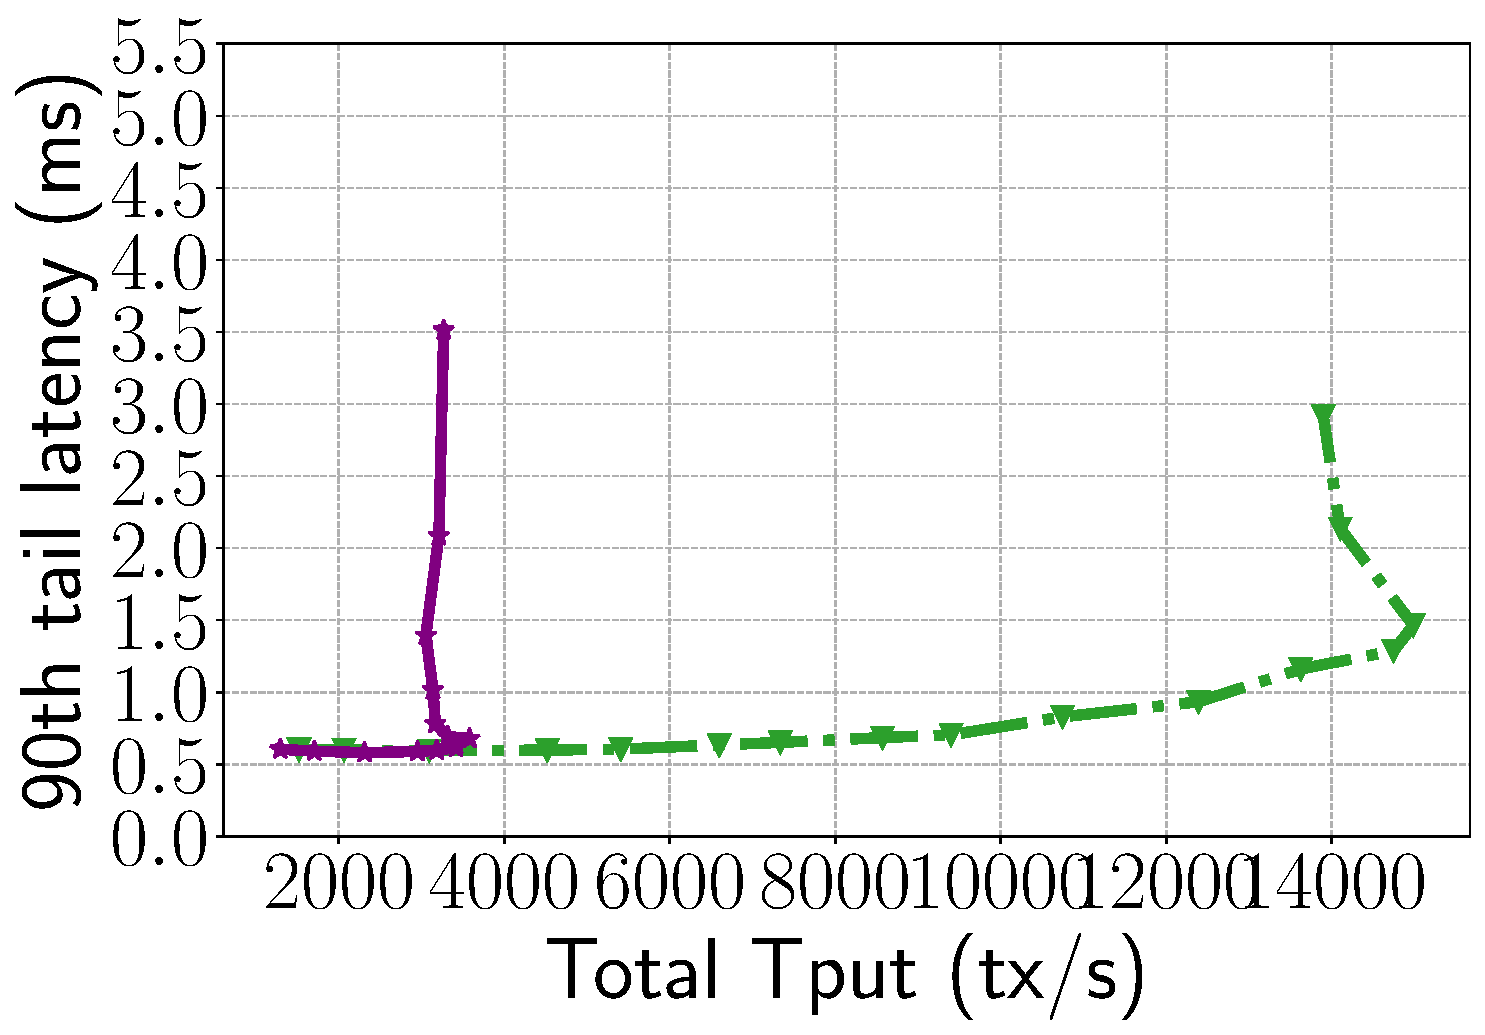
\includegraphics[width=0.45\columnwidth]{eval-figs/spanner_lat_tput.pdf}
	}
	\hfill 
	\subfloat[\footnotesize Abort Rate.\label{fig:spanner:overview:abort:breakdown}]{
		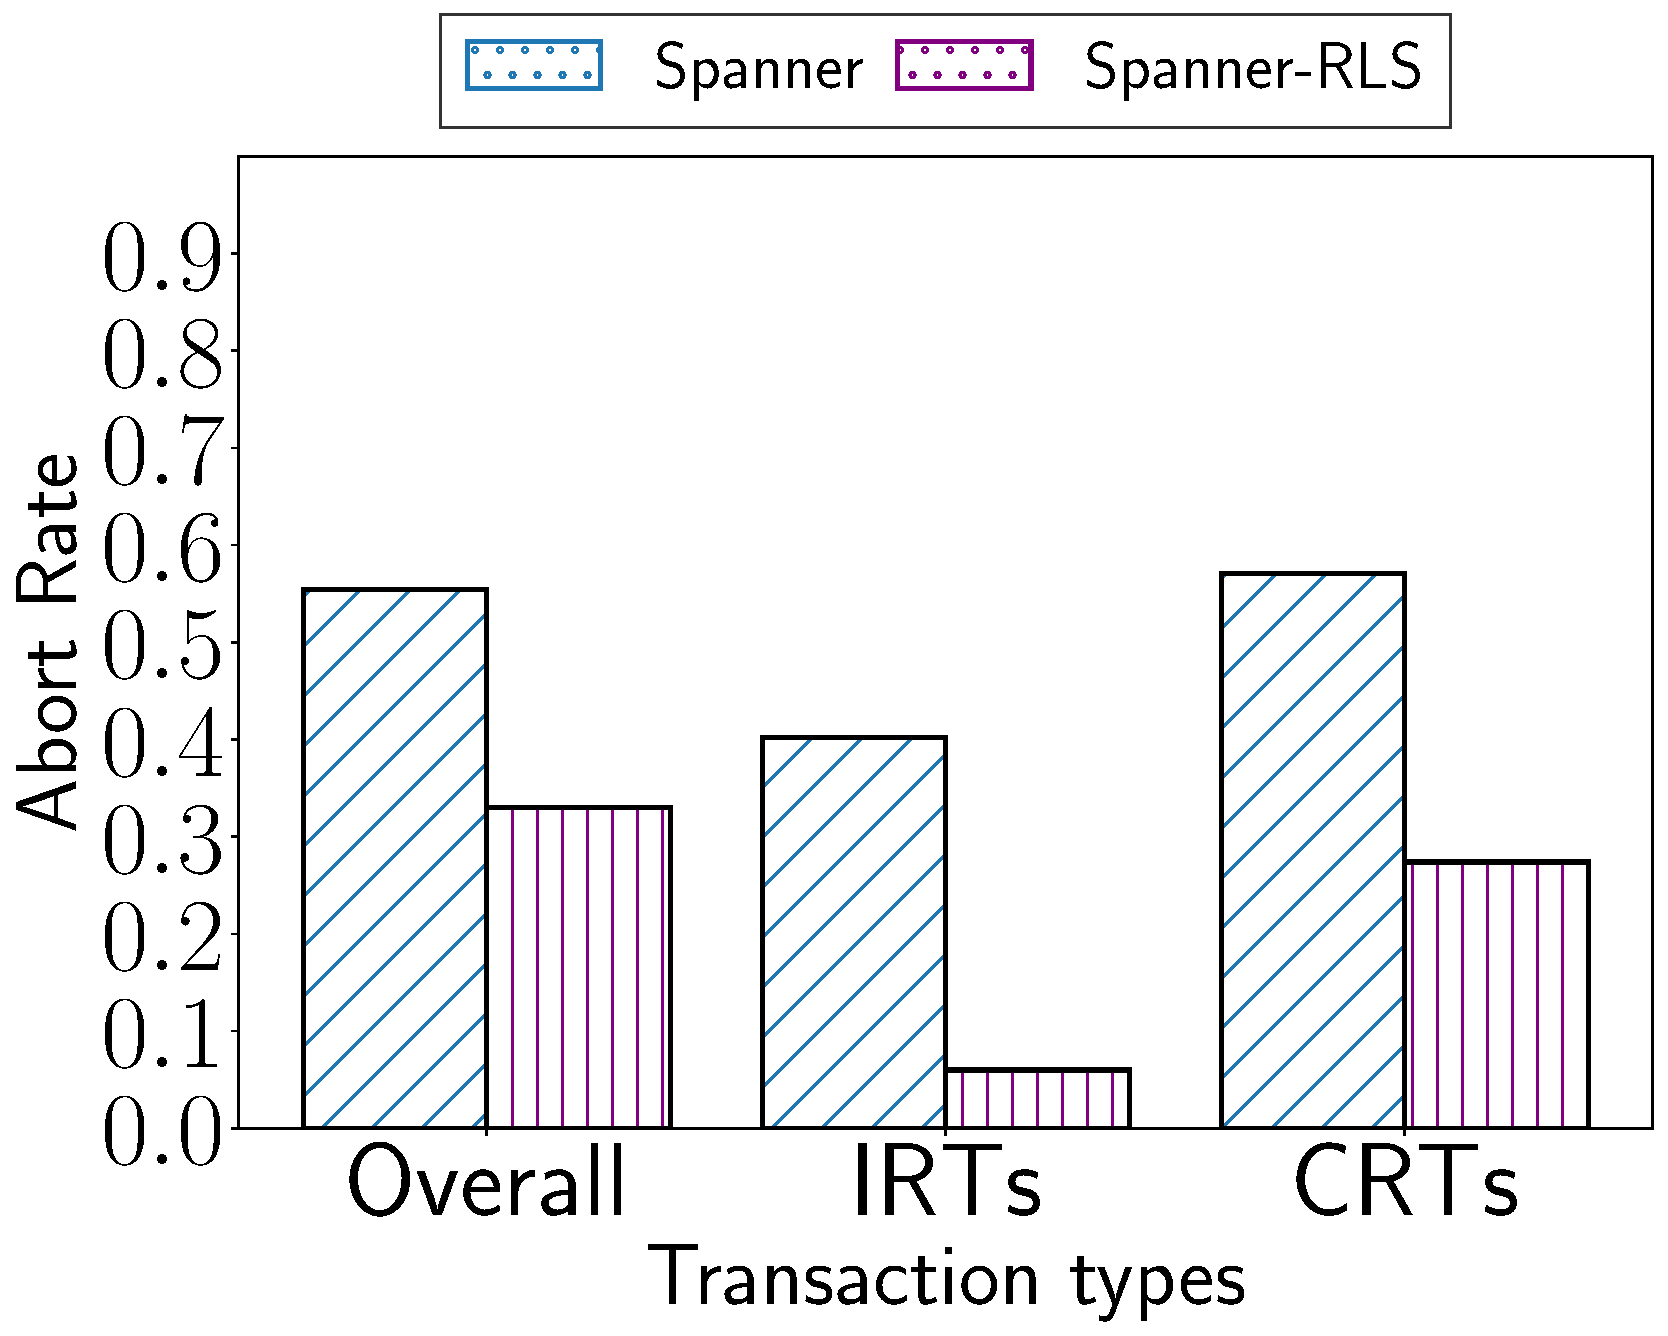
\includegraphics[width=0.45\columnwidth]{eval-figs/spanner_latency_waitdie.pdf}
	}
	\caption{Overall performance and abort rate of Spanner and Spannner-RLS on YCSB-T (default setting) using \texttt{NO\_WAIT}.}\label{fig:eval:spanner:overall:abort}
\end{figure}

\subsection{Evaluation and Discussion}\label{sec:spanner:eval}

\subsubsection{Experimental Setups} We implemented Spanner-RLS in C++ utilizing the third-party implementation~\cite{tapir:github} since the original version of Spanner is not open-sourced. We employed \texttt{libevent} for message passing between processes on distinct nodes and between threads in the same process. Transactions were implemented as stored procedures containing read and write operations over a set of keys.



\noindent\textbf{Cluster Setups.} All experiments were conducted on our cluster comprising $10$ machines, each with a 2.60GHz Intel E5-2690 CPU with 24 cores, 40Gbps NIC, and 64GB memory. We executed each data node (shard) in a docker container and utilized tc~\cite{linux:tc} to regulate the RTT among nodes. The server ran on the Ubuntu 18.04 operating system.


\noindent\textbf{Deployments.} To simulate a multi-region deployment, we abstracted each server as an individual region. Subsequently, We set the cross-region round-trip latency as $50ms$ using tc, aligning with the real-world statistics~\cite{azure:latency}. We partitioned the database into $300$ data shards, with each region containing $30$ data shards and a replication level of $3$, alongside transaction managers. By default, we utilized $40$ clients per region to attain the peak throughput for both Spanner and Spanner-RLS. 

\noindent\textbf{Workloads.} We employed the standard YCSB-T benchmark for our evaluation. We generated a total of $3,000,000$ keys, distributing $100,000$ keys per shard. Each transaction had $10$ operations, encompassing $5$ read operations and $5$ read-modify-write operations. By default, we tuned the percentage of CRTs to be $10\%$ and varied the amount of contention in the system by choosing keys according to a Zipf distribution with a Zipf coefficient = $0.75$ (medium and high contention). Each of our experiments lasted 3 minutes, with the first $30s$ and the last $30s$ excluded from results to avoid performance fluctuations during start-up and cool-down.

\noindent\textbf{Deadlock Mechanisms.} We considered two different deadlock mechanisms in our evaluation since these mechanisms impart different scopes to how RLS benefits Spanner.

\begin{figure}[t]
	\centering
	\subfloat[\footnotesize Overview\label{fig:spanner:overview:wait}]{
	   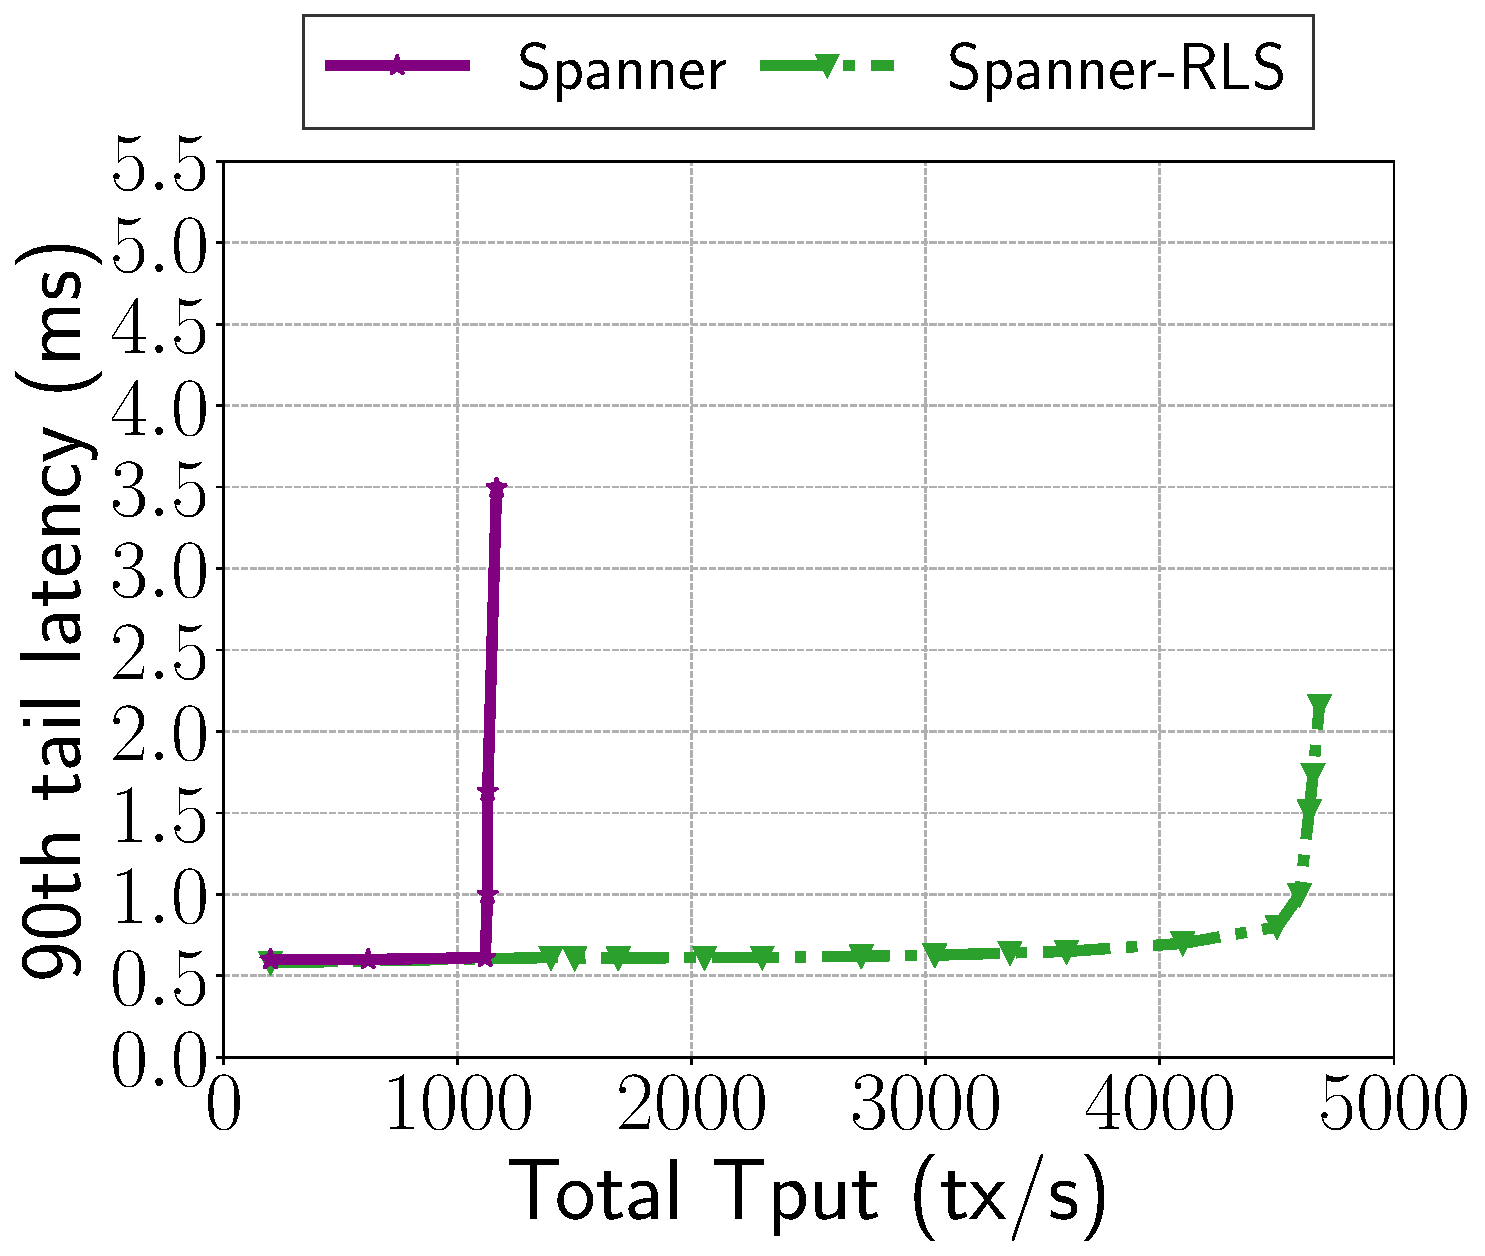
\includegraphics[width=0.45\columnwidth]{eval-figs/spanner_lat_tput_waitdie.pdf}
	}
	\hfill
	\subfloat[\footnotesize Tail latency.\label{fig:spanner:overview:wait:breakdown}]{
		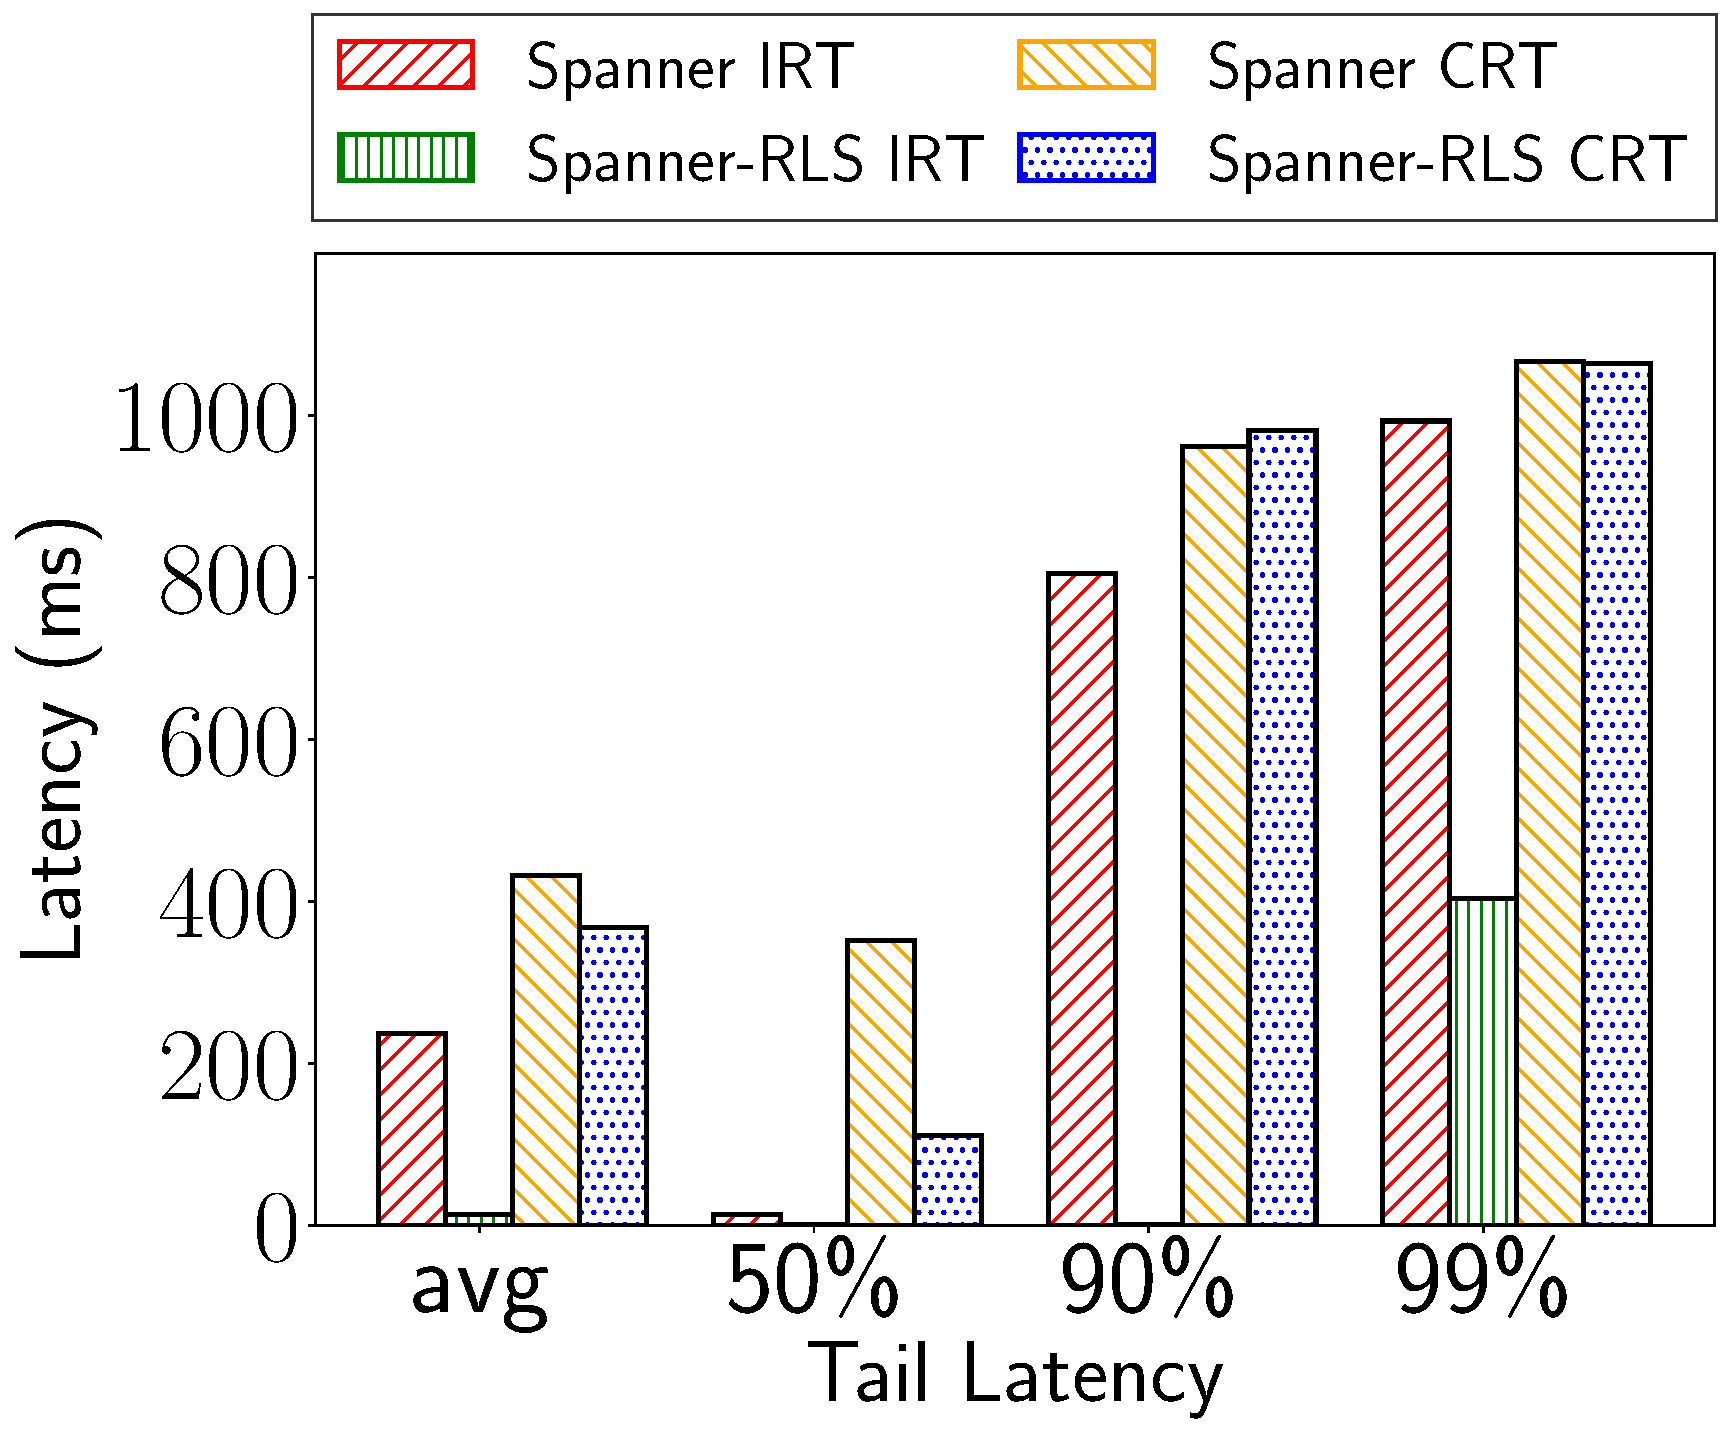
\includegraphics[width=0.45\columnwidth]{eval-figs/spanner_abortrate.pdf}
	}
	\caption{Overall performance and latency of Spanner and Spanner-RLS  on YCSB-T (default setting) using \texttt{WAIT\_DIE}.}\label{fig:eval:spanner:overall:wait}
\end{figure}


\begin{figure*}[t]
	\centering
	
\includegraphics[width=2\columnwidth]{eval-figs/legend_Spanner.png}
	\vspace{1pt}
	\subfloat[\footnotesize Impact of Concurrency\label{fig:spanner:concurrency:abort}]{
		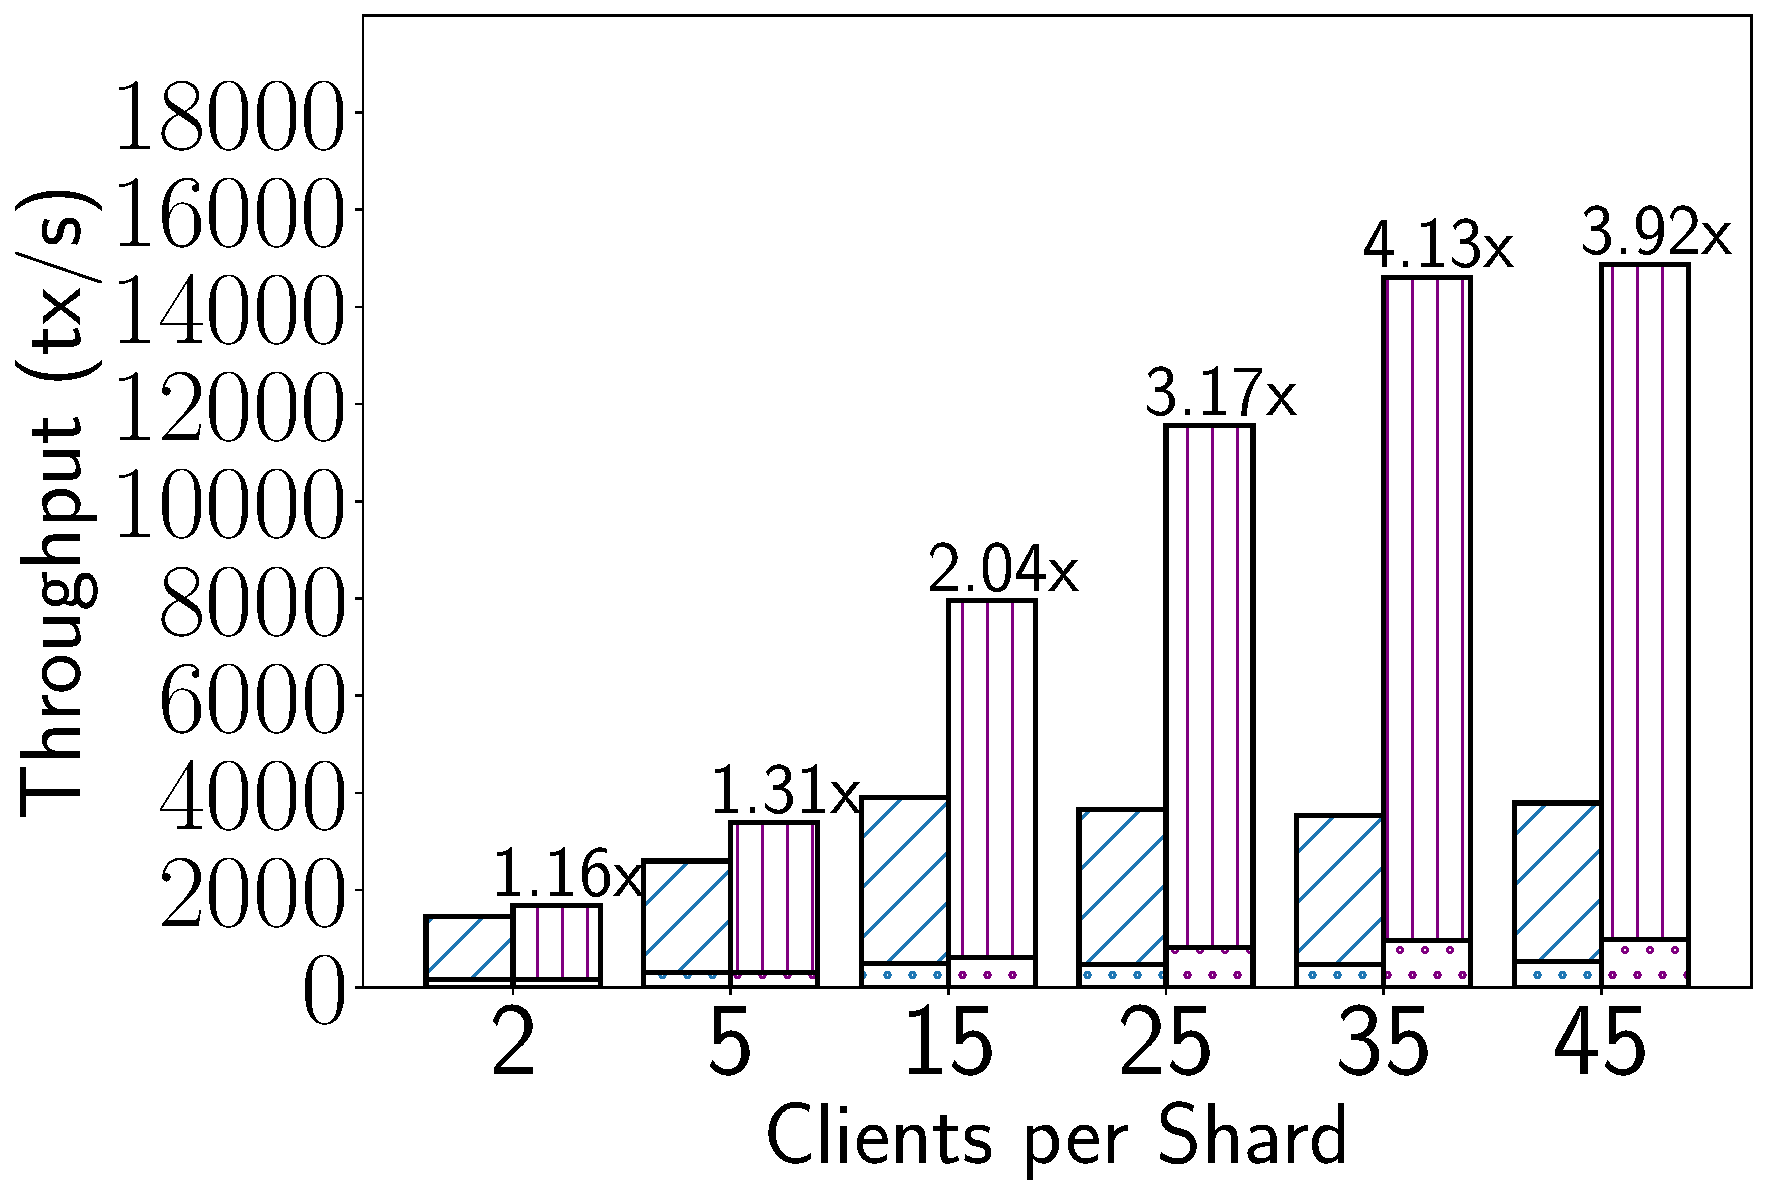
\includegraphics[width=0.48\columnwidth]{eval-figs/spanner_tput_client.pdf}
	}
	\hfill
	\subfloat[\footnotesize Impact of CRT\label{fig:spanner:crt:abort}]{
 	    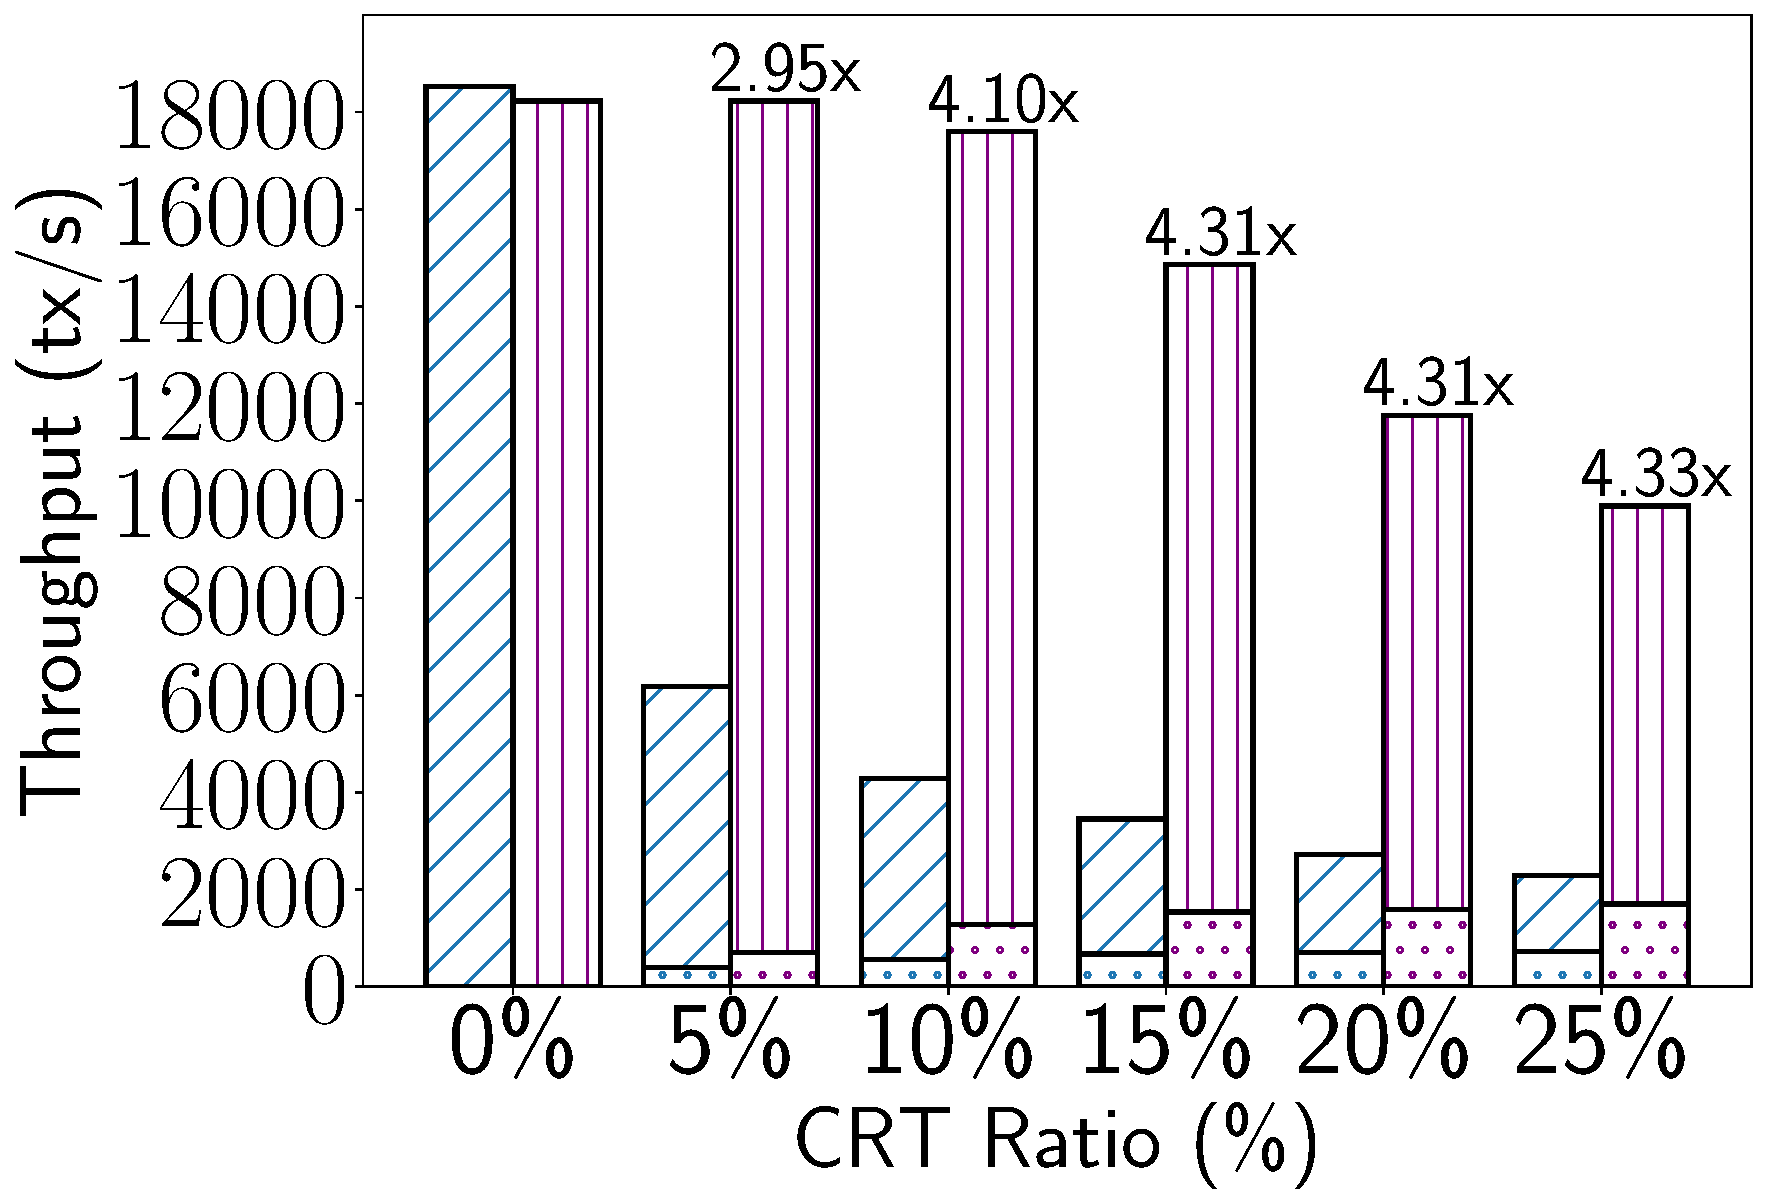
\includegraphics[width=0.48\columnwidth]{eval-figs/spanner_tput_crt.pdf}
	}
	\hfill
	\subfloat[\footnotesize Impact of RTT\label{fig:spanner:rtt:abort}]{
  	   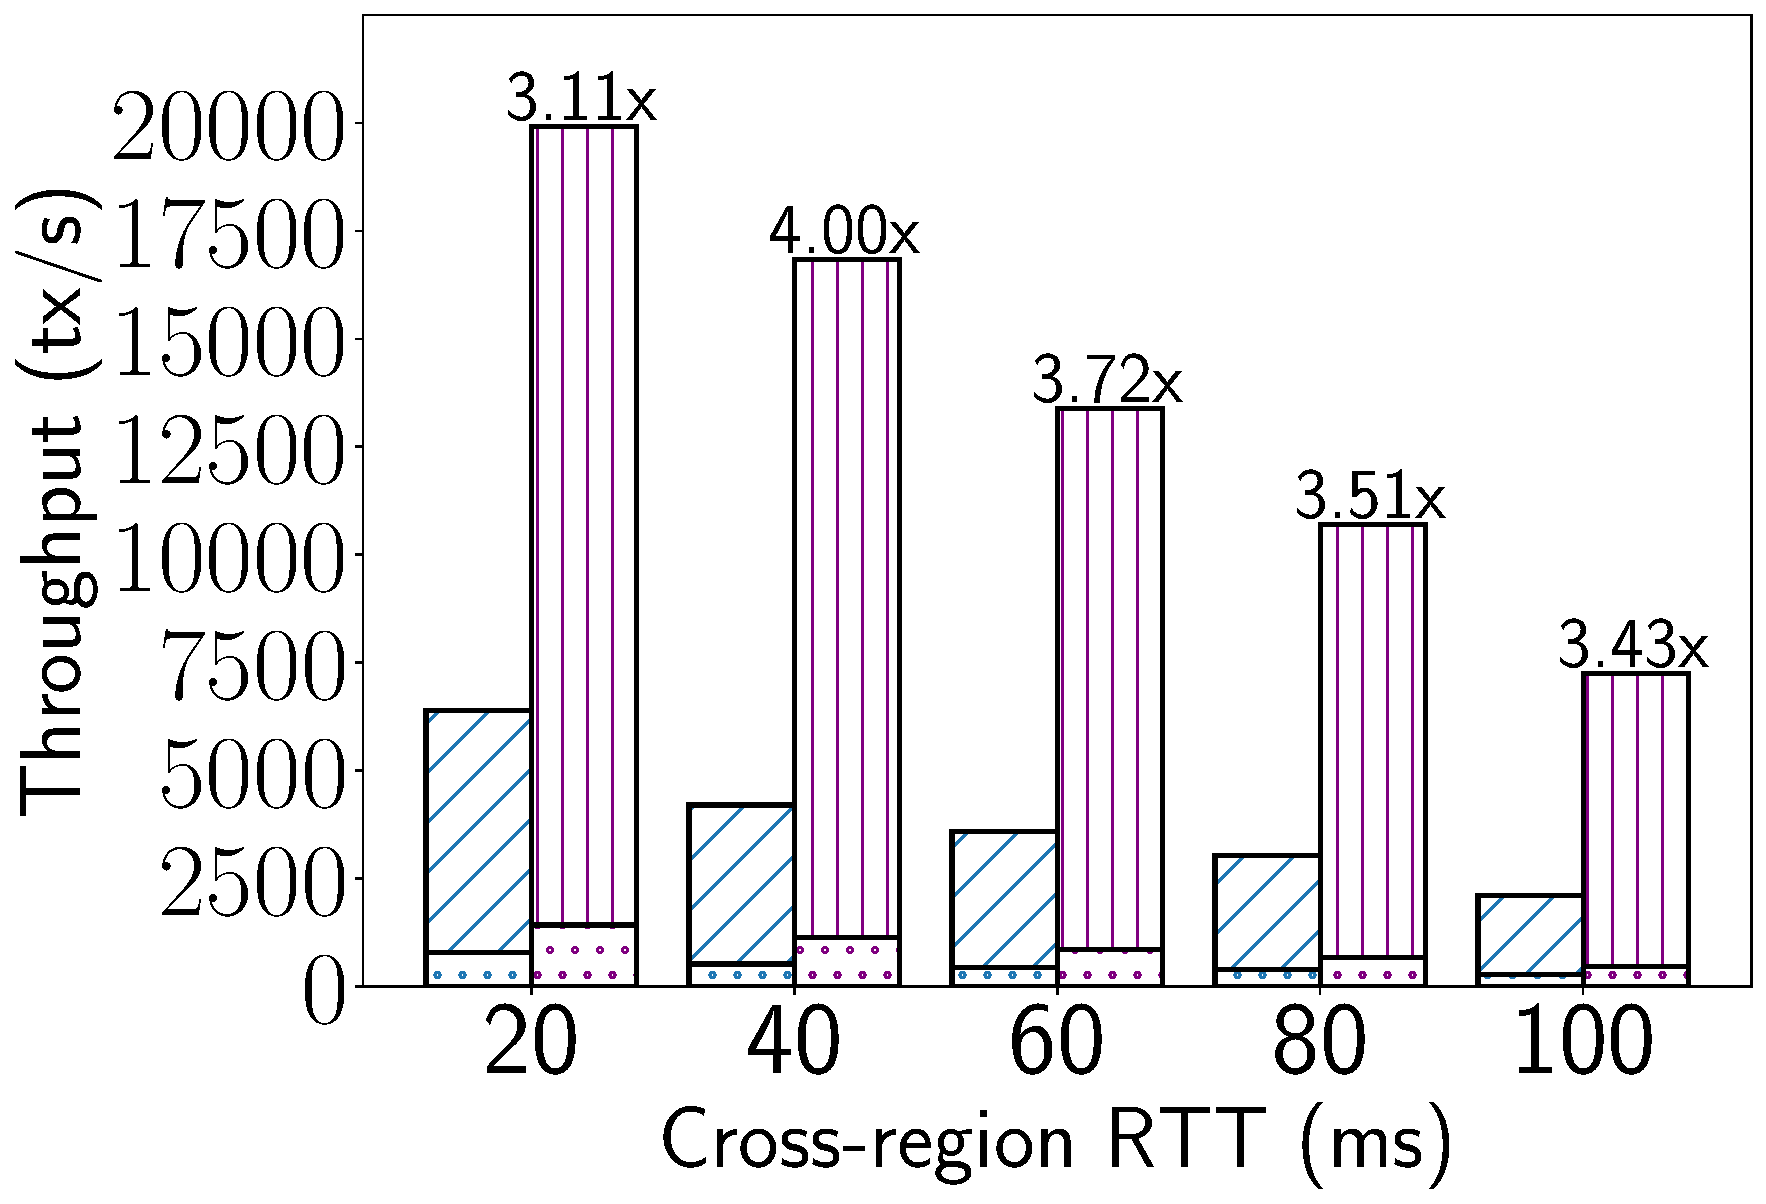
\includegraphics[width=0.48\columnwidth]{eval-figs/spanner_tput_rtt.pdf}
	}
	\hfill
	\subfloat[\footnotesize Impact of Conflicts\label{fig:spanner:zipf:abort}]{
        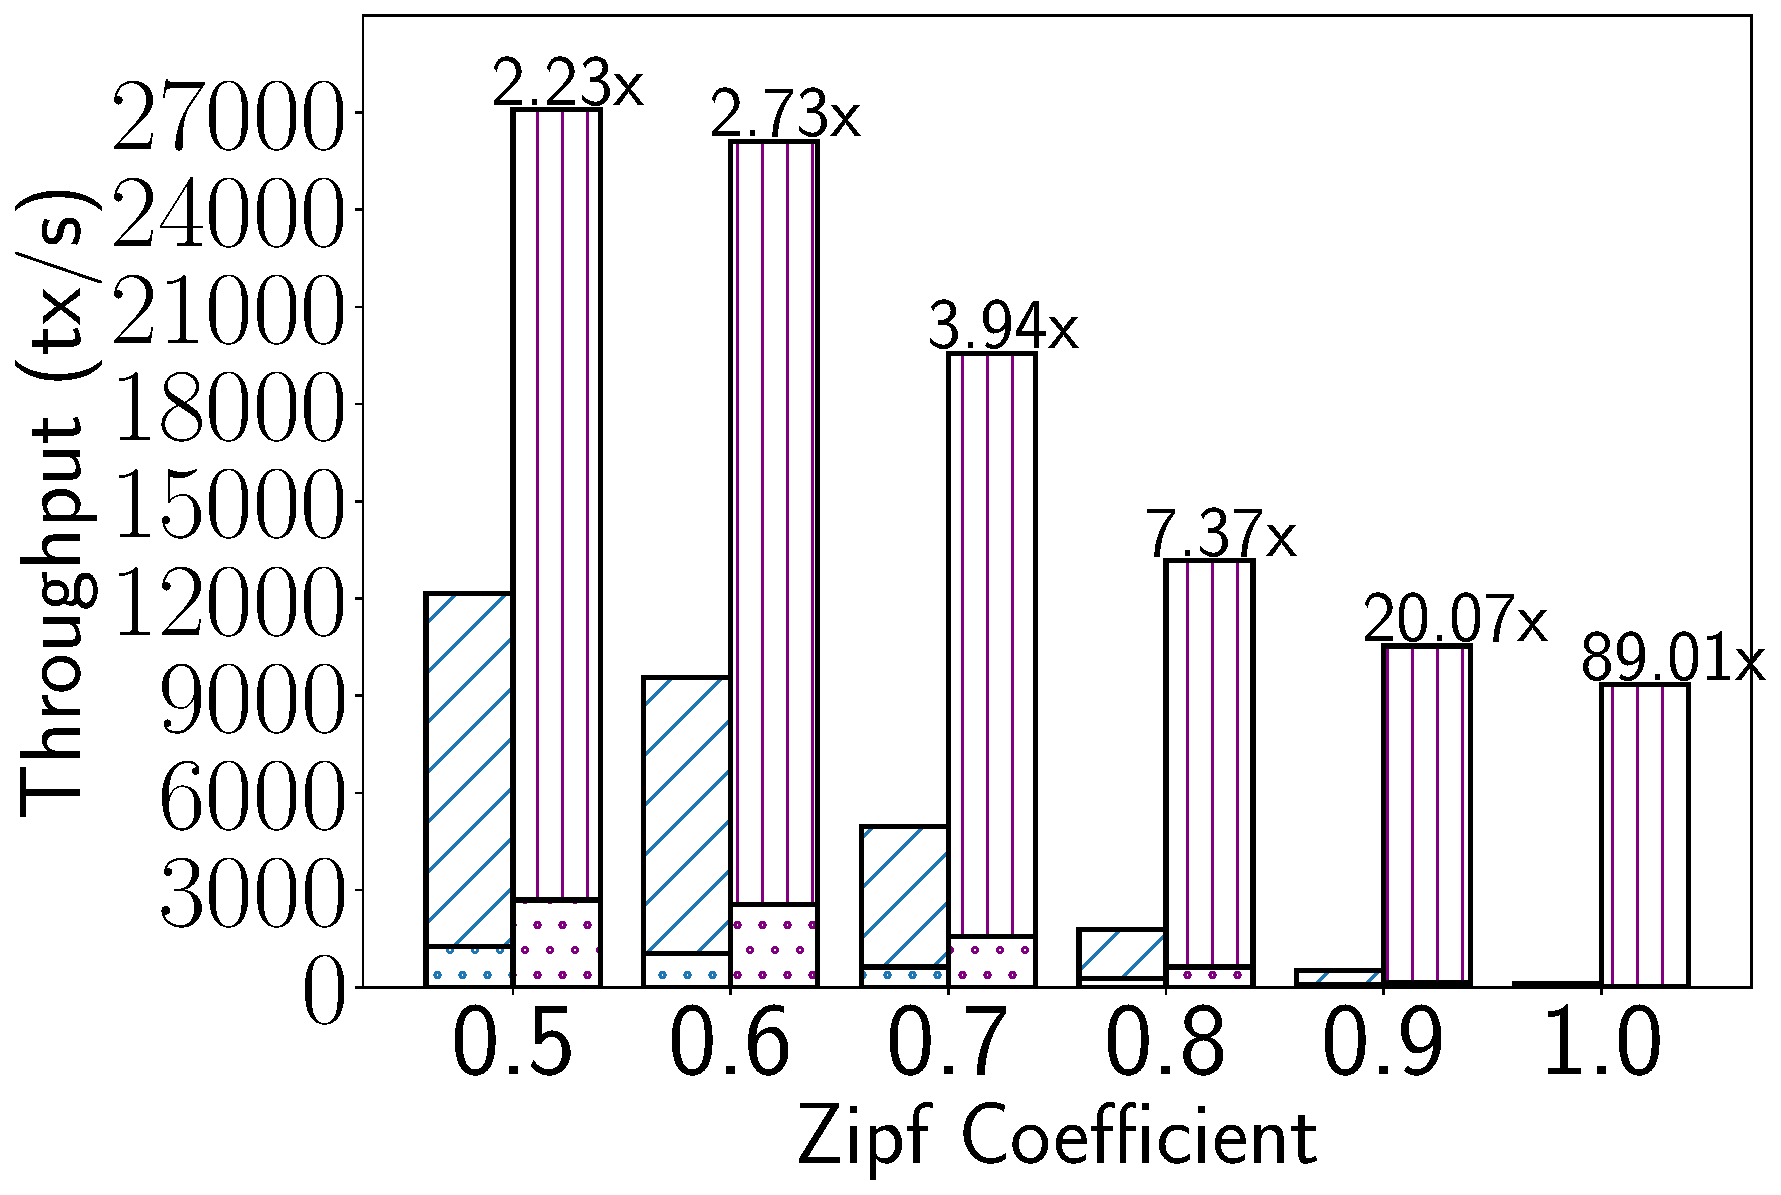
\includegraphics[width=0.48\columnwidth]{eval-figs/spanner_tput_zipf.pdf}
	}

	\caption{Performance of Spanner and Spanner-RLS on YCSB-T with different experimental parameters using \texttt{NO\_WAIT}.}\label{fig:eval:spanner:abort}
% \vspace{10pt}
\end{figure*}

\begin{figure*}[t]
	\centering
	
\includegraphics[width=2\columnwidth]{eval-figs/legend_Spanner.png}
	\vspace{1pt}
	\subfloat[\footnotesize Impact of Concurrency\label{fig:spanner:concurrency:wait}]{
		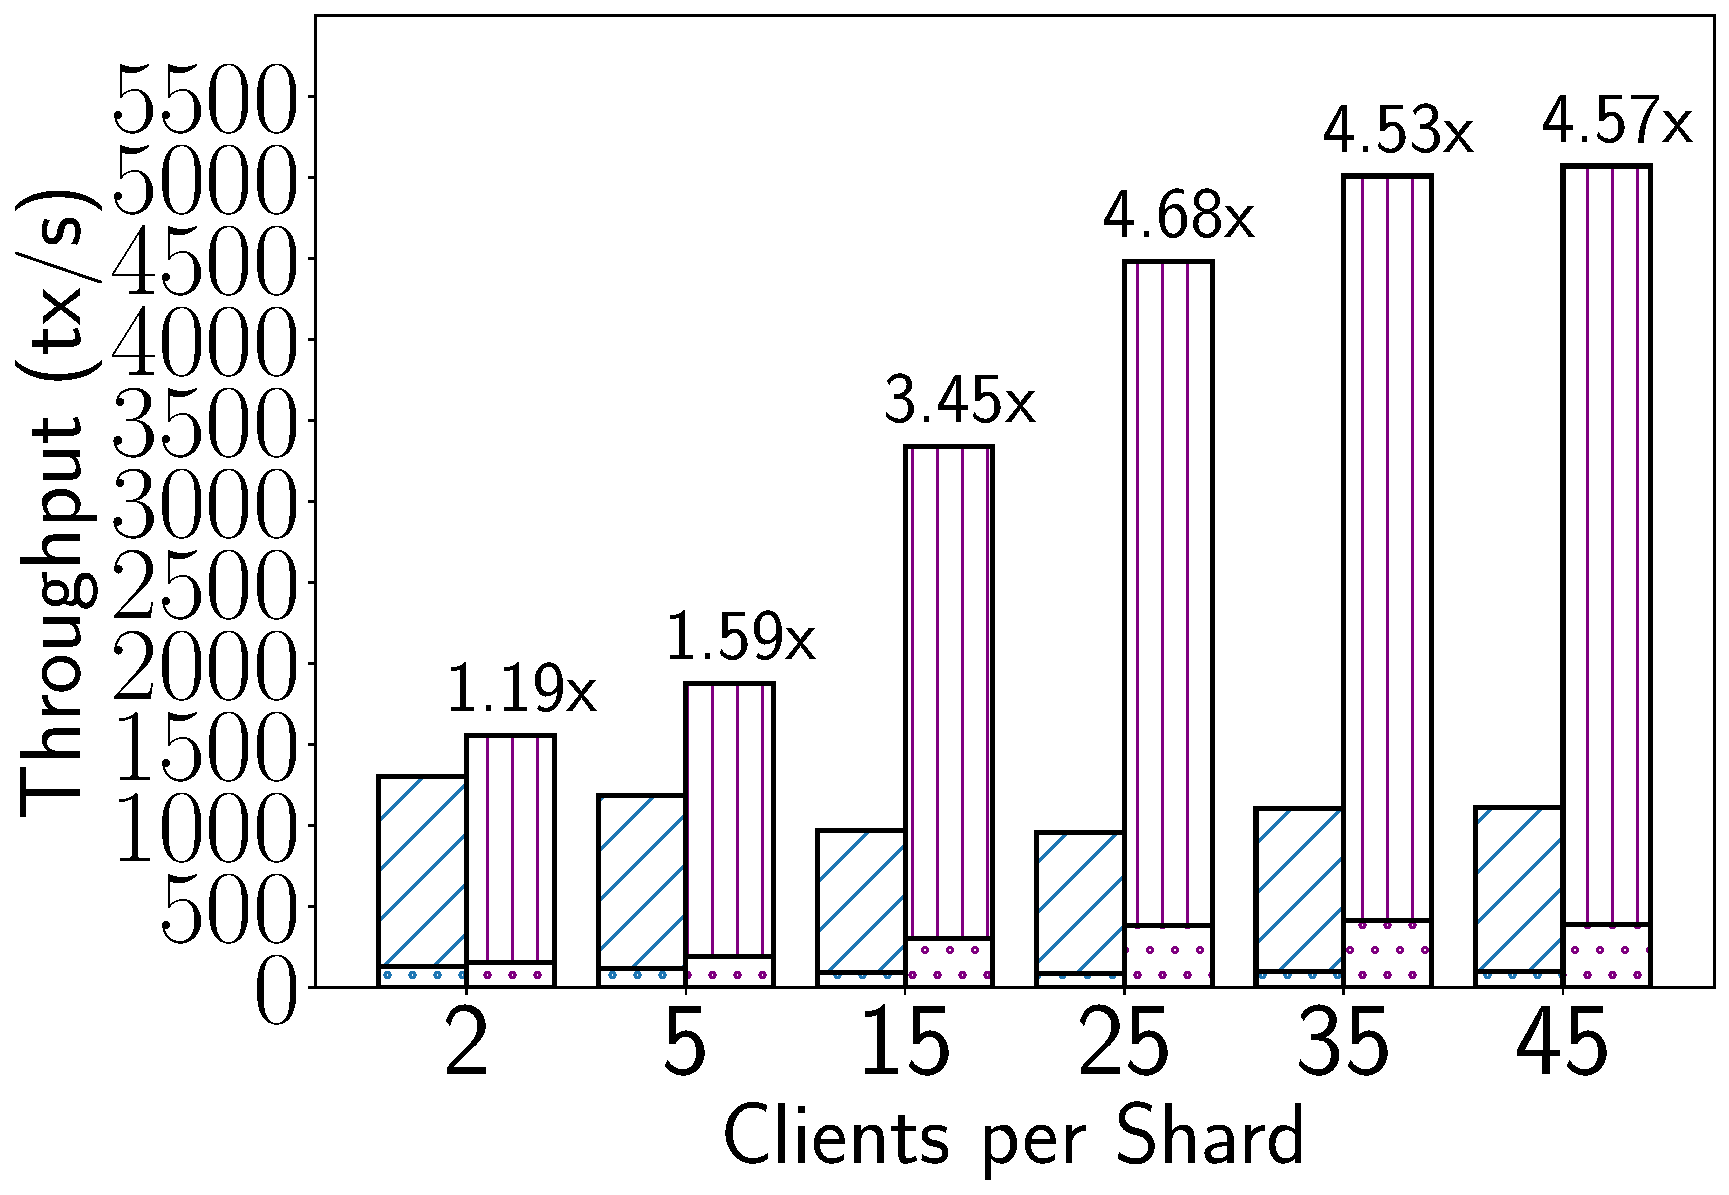
\includegraphics[width=0.23\textwidth]{eval-figs/spanner_tput_client_waitdie.pdf}
	}
	\hfill
	\subfloat[\footnotesize Impact of CRT\label{fig:spanner:crt:wait}]{
 	    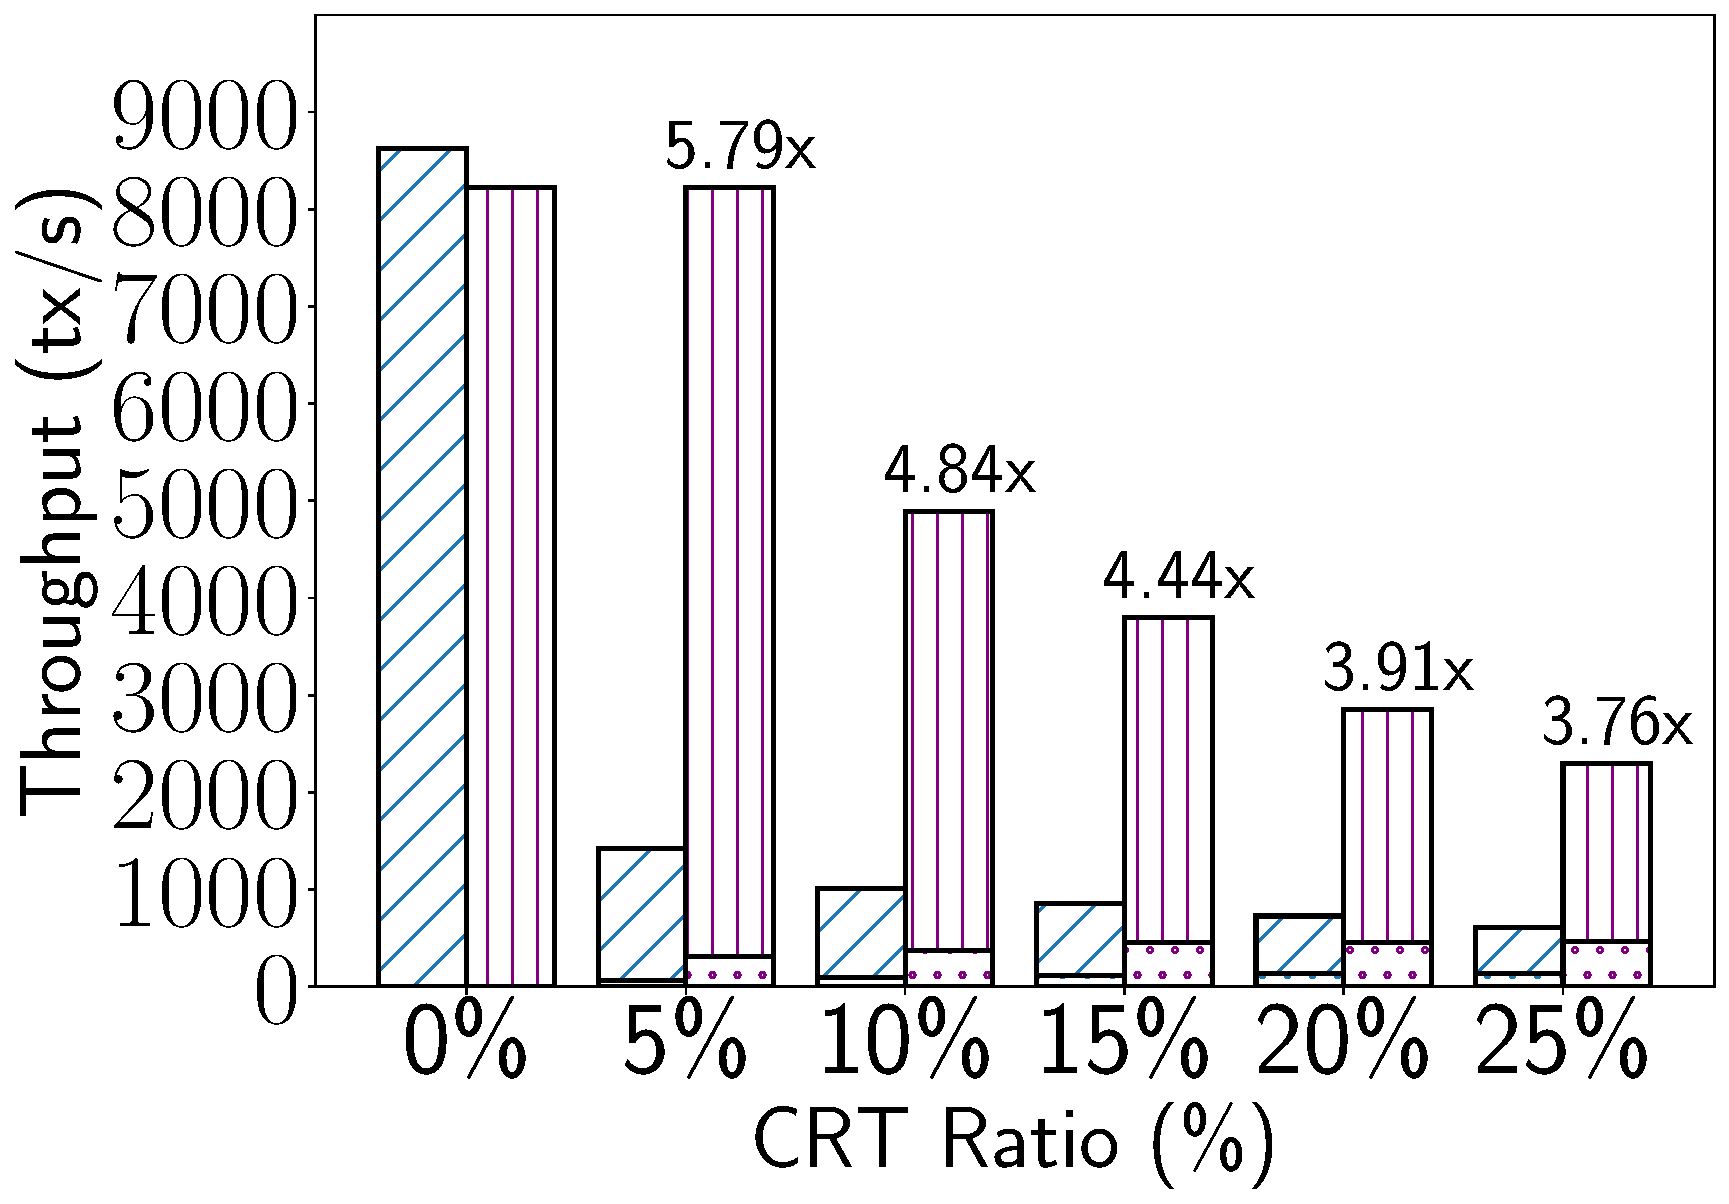
\includegraphics[width=0.23\textwidth]{eval-figs/spanner_tput_crt_waitdie.pdf}
	}
	\hfill
	\subfloat[\footnotesize Impact of RTT\label{fig:spanner:rtt:wait}]{
  	   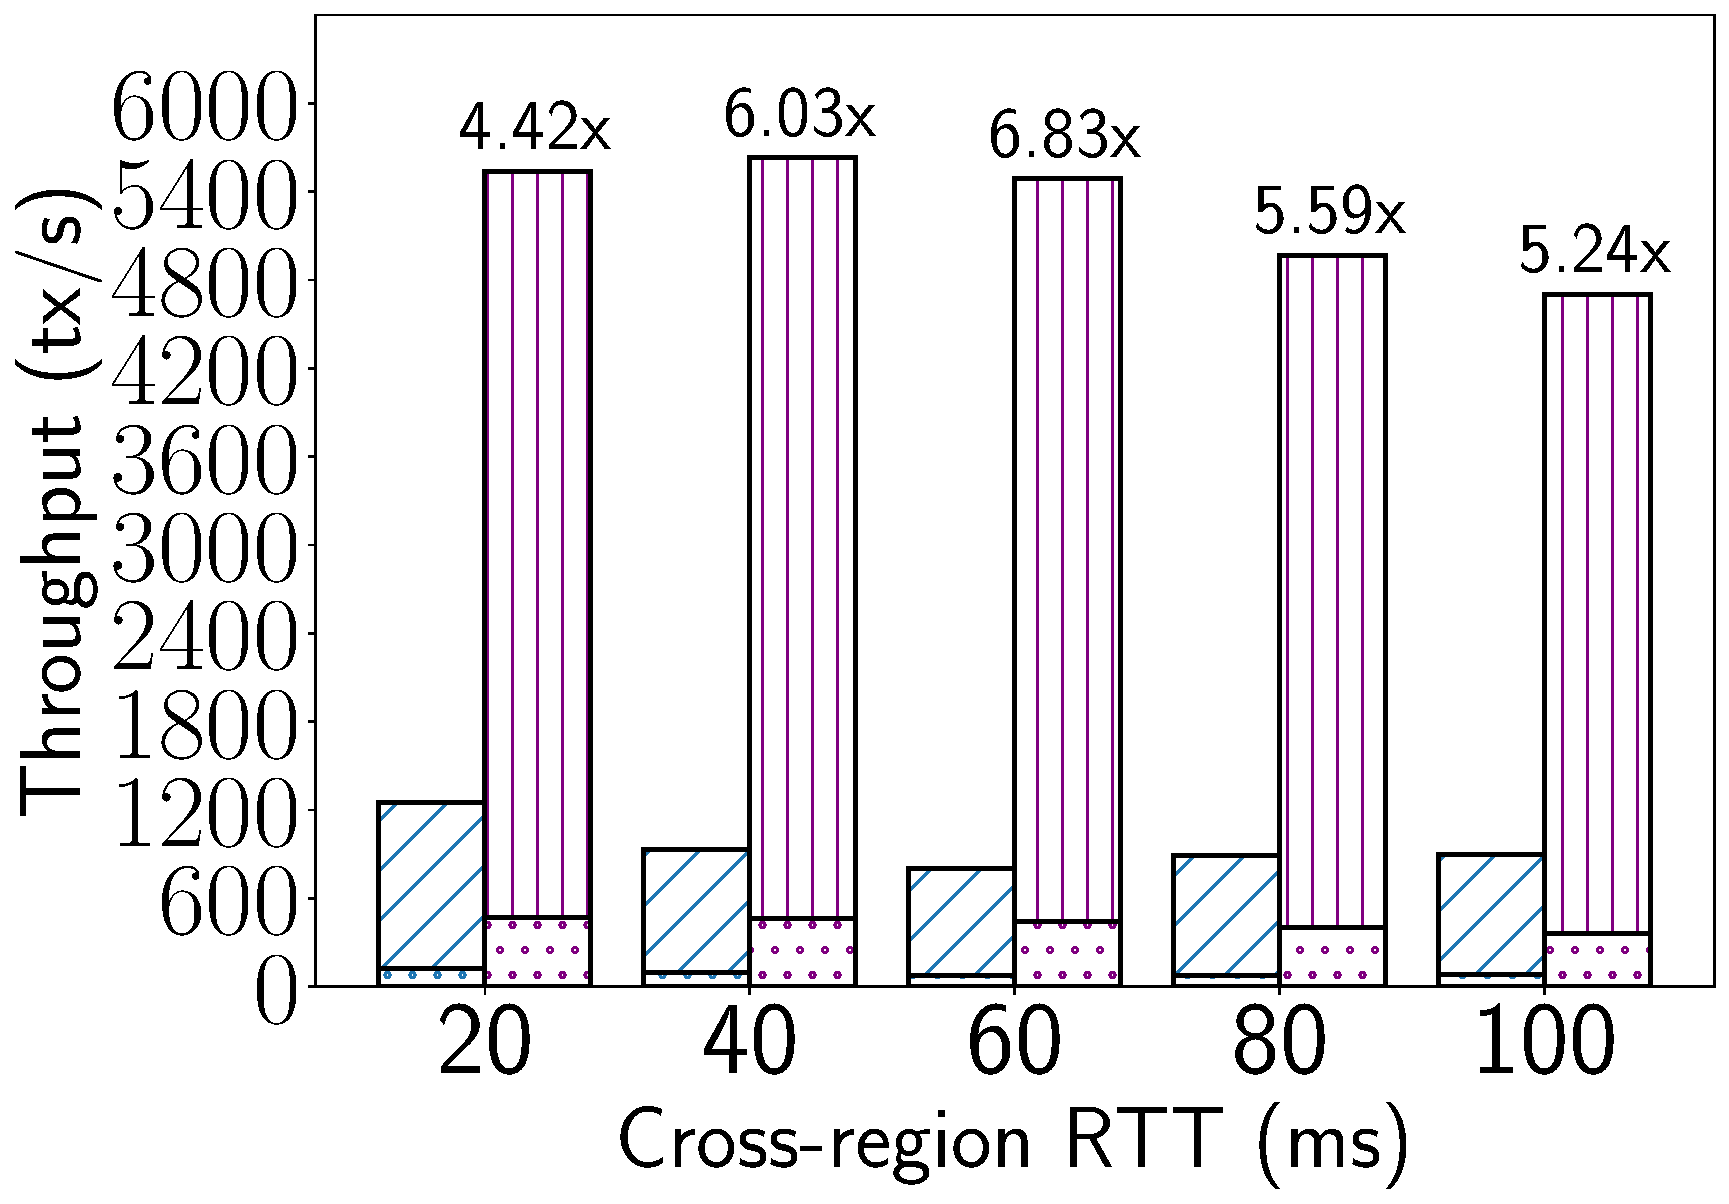
\includegraphics[width=0.23\textwidth]{eval-figs/spanner_tput_rtt_waitdie.pdf}
	}
	\hfill
	\subfloat[\footnotesize Impact of Conflicts\label{fig:spanner:zipf:wait}]{
        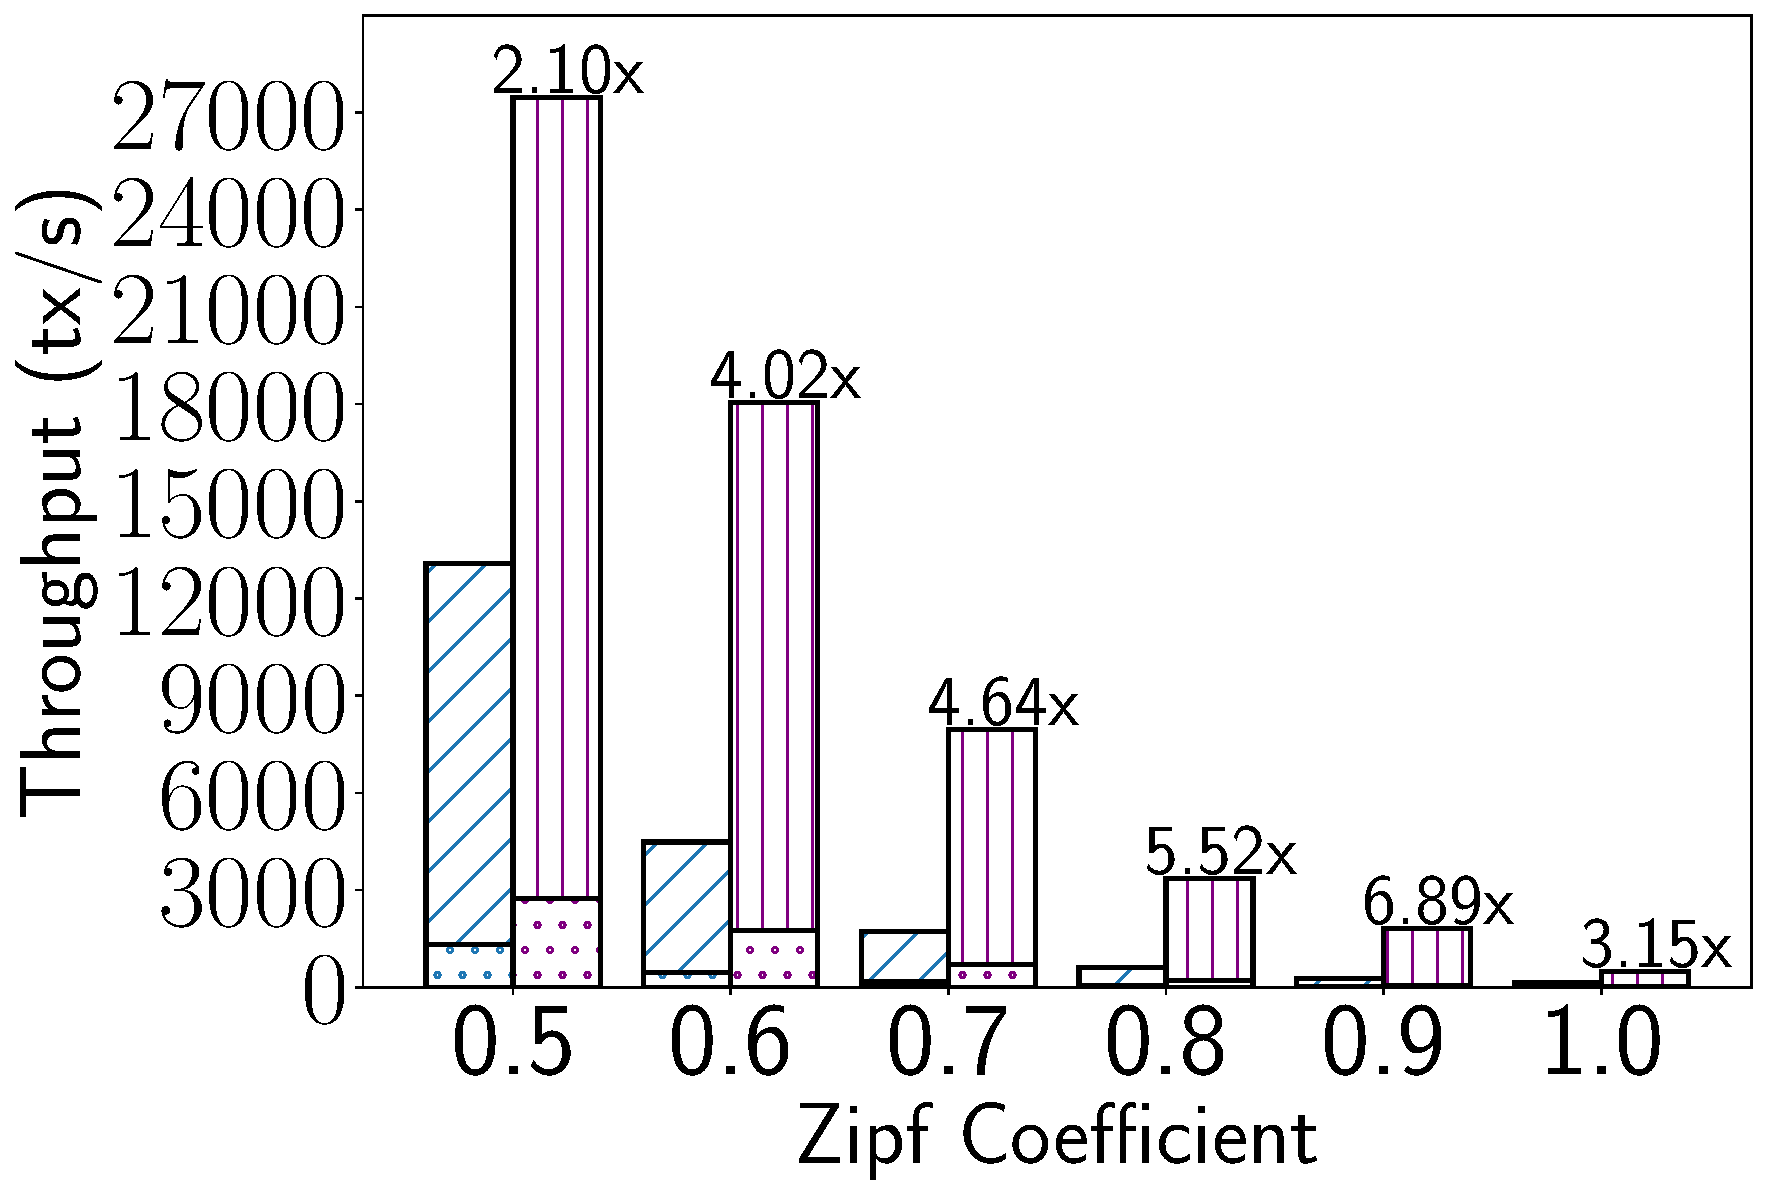
\includegraphics[width=0.23\textwidth]{eval-figs/spanner_tput_zipf_waitdie.pdf}
	}
  
	\caption{Performance of Spanner and Spanner-RLS on YCSB-T with different experimental parameters using \texttt{WAIT\_DIE}.}\label{fig:eval:spanner:wait}
	\vspace{10pt}
\end{figure*}

\begin{itemize}[leftmargin=*, itemsep=1.5pt]
    \setlength{\itemsep}{0pt}
    \setlength{\parsep}{0pt}
    \setlength{\parskip}{0pt}
\item \textbf{\texttt{NO\_WAIT.}} When using this deadlock mechanism, if a lock request is denied, the database will immediately abort the requesting transaction, and the client will retire the transaction. 
\item \textbf{\texttt{WAIT\_DIE.}} Unlike \texttt{NO\_WAIT}, \texttt{WAIT\_DIE} allows a transaction to wait for the requested lock if the transaction is older than the one that holds the lock. Otherwise, the transaction is forced to abort and will be retired by the client. 
\end{itemize}

We do not consider other deadlock mechanisms since they are either subsumed by the two mechanisms or will incur significant overhead in a multi-region deployment. 
For instance, deadlock detection necessitates a centralized deadlock detector for cycle detection, which can be expensive due to cross-region communication.

\subsubsection{Performance Overview} 

We first evaluated the performance under the default setting. For an apple-to-apple comparison, we refrained from using prior knowledge of read and write sets in our experiments, even though the read and compose set of YCSB-T can be revealed before execution. As shown in \fig{fig:spanner:overview:abort}  and \fig{fig:spanner:overview:wait}, Spanner-RLS significantly outperformed Spanner on YCSB-T. In particular, Spanner-RLS achieved $3.95\times$ and $4.27\times$ higher peak throughput when utilizing \texttt{NO\_WAIT} and \texttt{WAIT\_DIE}, respectively. Spanner-RLS's $90th$ resembled that of Spanner, essentially representing the IRTs latency. We observed that employing the \texttt{NO\_WAIT} mechanism resulted in substantially higher throughput than using \texttt{WAIT\_DIE}, given the default workload's write-intensive nature with medium contention.

To comprehend how our new design contributes to performance improvement, we gathered data on the abort rate for \texttt{NO\_WAIT} and tail latency for \texttt{WAIT\_DIE} when both Spanner and Spanner-RLS achieved the peak throughput. \fig{fig:spanner:overview:abort:breakdown} and \fig{fig:spanner:overview:wait:breakdown} illustrate the results. 

Regarding \texttt{NO\_WAIT}, Spanner-RLS can efficiently reduce the abort rate for both IRTs and CRTs. The overall abort ratedecreased from $56\%$ to $33\%$ (i.e., $41.1\%$ reduction). In particular, Spanner-RLS achieved a  more significant reduction for IRTs (from $40\%$ to $6\%$) due to the ``non-blocking'' property in IRT coordination and commitment. It's worth mentioning that the $6\%$ abort rate was only caused by the contention among IRTs. Meanwhile, the abort rate of CRTs also saw a reduction. However, compared to IRTs, CRTs still exhibited a much higher abort rate (i.e., $27.42\%$) due to the larger contention footprint.

For \texttt{WAIT\_DIE}, Spanner-RLS achieved a significantly lower average latency for IRTs, while the average latency of CRTs was roughly the same as in Spanner. This is attributed to the fact that in Spanner-RLS, an IRT will never be blocked by CRTs. The results on $50th$ and $90th$ latency support this assertion. Both Spanner and Spanner-RLS exhibited low $50th$ latency, while the $90th$ latency of Spanner and Spanner-RLS was $805ms$ and $1.4ms$, respectively. The $99th$ latency of Spanner-RLS increased due to the queueing effect in the software stack. 

Next, we delve into understanding how Spanner-RLS and Spanner are affected by various workload parameters. These experiments were conducted using YCSB's APIs as they offer flexibility in configuration.



\subsubsection{Impact of Concurrency} We first compare the performance of Spanner-RLS and Spanner under various concurrencies. As illustrated in \fig{fig:spanner:concurrency:abort} and \fig{fig:spanner:concurrency:wait}, Spanner's throughput reached saturation rapidly as the number of clients increased. Consequently, the peak throughput of Spanner was $3911$ and $1181$ transactions per second using \texttt{No\_WAIT} and \texttt{WAIT\_DIE}, respectively. In contrast, Spanner-RLS could serve more clients and achieve a substantially higher peak throughput.

\subsubsection{Impact of CRT Ratio} We studied the impact of the CRT ratio by fine-tuning the workload generation. As shown in \fig{fig:spanner:crt:abort} and \fig{fig:spanner:crt:wait}, when CRTs were enabled, Spanner experienced 
severe performance degradation (e.g., throughput dropping from $18526$ transactions per second to $6184$ transactions per second when the CRT ratio increased from $0\%$ to $5\%$), aligning with our discussion in \chref{sec:intro} and \chref{sec:background:geo}. In contrast, Spanner-RLS's performance degraded slightly, attributed to the elimination of cross-region costs for IRTs. In scenarios where all transactions were IRTs (i.e., a special case in our experiments), Spanner-RLS demonstrated slightly lower throughput than Spanner due to the cost for extra steps in concurrency control (i.e., checking transaction types even if all transactions are IRTs). With a continuous increase in CRT ratios, the throughput of Spanner and Spanner-RLS decreased due to cross-region communication costs. In practice, the CRT ratio of workloads should not be too high since the cost of CRT itself is still relatively high compared to IRTs. Real-world workloads show good data locality under multi-region deployment (\chref{sec:background:deployment}), facilitating low-latency data access.



\subsubsection{Impact of Cross-Region RTT} Next, we studied the impact of the cross-region network delays, a critical factor affecting the overall cost of CRTs. Larger cross-region network delays generally result in longer transaction coordination and commit times for CRTs. The results, illustrated in \fig{fig:spanner:rtt:abort} and \fig{fig:spanner:rtt:wait}, clearly indicate that Spanner-RLS outperforms Spanner regardless of the cross-region network delays. In fact, Spanner-RLS demonstrates more when the network delays are moderate (e.g., $40s$ and $60s$ for a cross-region network round trip). In addition, the network delay amplifies the advantages of Spanner-RLS while also affecting Spanner-RLS's CRTs, causing a drop in throughput from $1429$ transactions per second to $476$ transactions per second as the network delay increased from $20$ seconds to $100$ seconds using \texttt{NO\_WAIT}.



\subsubsection{Impact of Contention} In our final experiment, we compared the performance under various contention by adjusting the skewness of Zipf distribution in YCSB-T while keeping other parameters consistent with the default settings. The results depicted in \fig{fig:spanner:zipf:abort} and \fig{fig:spanner:zipf:wait} consistently show that the Spanner-RLS's throughput outperforms Spanner's across all levels of contention. This improvement stems from Spanner-RLS efficiently reducing the contention footprint by ordering IRTs and CRTs independently. As discussed in \chref{sec:background:geo}, the contention footprint of IRTs eliminates both ``coordination blocking'' and ``commit blocking'', which is extremely expensive in multi-region deployments. As expected by our analysis, Spanner-RLS gained larger margins under high contention. This is because, under high contention, IRTs in Spanner have more chance to be blocked by CRTs, leading to poor performance. It should be noted that the performance of Spanner-RLS also degraded due to the cost of acquiring locks, and \texttt{NO\_WAIT} consistently outperformed \texttt{WAIT\_DIE} since \texttt{WAIT\_DIE} suffers more from lock thrashing and timestamp allocation when the contention is higher.

\subsection{Takeaways}
By adhering to the principles of RLS, developers can significantly enhance the performance of Spanner. Spanner-RLS serves as a practical example, illustrating how RLS can assist multi-region databases in achieving an optimal balance between consistency and performance. Further enhancements in the performance of Spanner-RLS can be achieved by implementing advanced optimizations (e.g., a pre-write-log mechanism in RedT~\cite{zhang2023redt}), which is orthogonal to our paper. We believe our study on Spanner-RLS holds the potential to guide future research by encouraging researchers and developers to consider multi-level two-phase locking and two-phase commit. Even though the design of Spanner-RLS may not be directly applicable to other strictly serializable concurrency protocols due to potential differences in transaction coordination mechanisms, the fundamental concept of RLS remains applicable.

